% Options for packages loaded elsewhere
\PassOptionsToPackage{unicode}{hyperref}
\PassOptionsToPackage{hyphens}{url}
\PassOptionsToPackage{dvipsnames,svgnames,x11names}{xcolor}
\documentclass[
  12,
]{article}
\usepackage{xcolor}
\usepackage[margin=1in]{geometry}
\usepackage{amsmath,amssymb}
\setcounter{secnumdepth}{-\maxdimen} % remove section numbering
\usepackage{iftex}
\ifPDFTeX
  \usepackage[T1]{fontenc}
  \usepackage[utf8]{inputenc}
  \usepackage{textcomp} % provide euro and other symbols
\else % if luatex or xetex
  \usepackage{unicode-math} % this also loads fontspec
  \defaultfontfeatures{Scale=MatchLowercase}
  \defaultfontfeatures[\rmfamily]{Ligatures=TeX,Scale=1}
\fi
\usepackage{lmodern}
\ifPDFTeX\else
  % xetex/luatex font selection
\fi
% Use upquote if available, for straight quotes in verbatim environments
\IfFileExists{upquote.sty}{\usepackage{upquote}}{}
\IfFileExists{microtype.sty}{% use microtype if available
  \usepackage[]{microtype}
  \UseMicrotypeSet[protrusion]{basicmath} % disable protrusion for tt fonts
}{}
\usepackage{graphicx}
\makeatletter
\newsavebox\pandoc@box
\newcommand*\pandocbounded[1]{% scales image to fit in text height/width
  \sbox\pandoc@box{#1}%
  \Gscale@div\@tempa{\textheight}{\dimexpr\ht\pandoc@box+\dp\pandoc@box\relax}%
  \Gscale@div\@tempb{\linewidth}{\wd\pandoc@box}%
  \ifdim\@tempb\p@<\@tempa\p@\let\@tempa\@tempb\fi% select the smaller of both
  \ifdim\@tempa\p@<\p@\scalebox{\@tempa}{\usebox\pandoc@box}%
  \else\usebox{\pandoc@box}%
  \fi%
}
% Set default figure placement to htbp
\def\fps@figure{htbp}
\makeatother
% definitions for citeproc citations
\NewDocumentCommand\citeproctext{}{}
\NewDocumentCommand\citeproc{mm}{%
  \begingroup\def\citeproctext{#2}\cite{#1}\endgroup}
\makeatletter
 % allow citations to break across lines
 \let\@cite@ofmt\@firstofone
 % avoid brackets around text for \cite:
 \def\@biblabel#1{}
 \def\@cite#1#2{{#1\if@tempswa , #2\fi}}
\makeatother
\newlength{\cslhangindent}
\setlength{\cslhangindent}{1.5em}
\newlength{\csllabelwidth}
\setlength{\csllabelwidth}{3em}
\newenvironment{CSLReferences}[2] % #1 hanging-indent, #2 entry-spacing
 {\begin{list}{}{%
  \setlength{\itemindent}{0pt}
  \setlength{\leftmargin}{0pt}
  \setlength{\parsep}{0pt}
  % turn on hanging indent if param 1 is 1
  \ifodd #1
   \setlength{\leftmargin}{\cslhangindent}
   \setlength{\itemindent}{-1\cslhangindent}
  \fi
  % set entry spacing
  \setlength{\itemsep}{#2\baselineskip}}}
 {\end{list}}
\usepackage{calc}
\newcommand{\CSLBlock}[1]{\hfill\break\parbox[t]{\linewidth}{\strut\ignorespaces#1\strut}}
\newcommand{\CSLLeftMargin}[1]{\parbox[t]{\csllabelwidth}{\strut#1\strut}}
\newcommand{\CSLRightInline}[1]{\parbox[t]{\linewidth - \csllabelwidth}{\strut#1\strut}}
\newcommand{\CSLIndent}[1]{\hspace{\cslhangindent}#1}
\setlength{\emergencystretch}{3em} % prevent overfull lines
\providecommand{\tightlist}{%
  \setlength{\itemsep}{0pt}\setlength{\parskip}{0pt}}
\usepackage{setspace}\doublespacing
\usepackage{indentfirst}
\usepackage{bookmark}
\IfFileExists{xurl.sty}{\usepackage{xurl}}{} % add URL line breaks if available
\urlstyle{same}
\hypersetup{
  pdftitle={Your Latex Template for Replication},
  pdfauthor={Your Name},
  colorlinks=true,
  linkcolor={Maroon},
  filecolor={Maroon},
  citecolor={Blue},
  urlcolor={blue},
  pdfcreator={LaTeX via pandoc}}

\title{Your Latex Template for Replication}
\usepackage{etoolbox}
\makeatletter
\providecommand{\subtitle}[1]{% add subtitle to \maketitle
  \apptocmd{\@title}{\par {\large #1 \par}}{}{}
}
\makeatother
\subtitle{Subtitle}
\author{Your Name}
\date{Date}

\begin{document}
\maketitle

\pagenumbering{gobble} 
\centerline{}
\pagenumbering{arabic}

\section{Introduction}\label{introduction}

This document provides the basic RMarkdown template using LaTeX for the
final replication project and (hopefully) your future work.

\subsection{Second Layer}\label{second-layer}

This is the second layer of Introduction. You can keep creating deeper
layers with more hashtags in front of the title.

\section{Mathematical Equations}\label{mathematical-equations}

\begin{itemize}
\item
  There are two modes for mathematical expressions: the \textbf{inline
  mode} and the \emph{display mode}. The first one is used to write
  formulas that are part of a text. The second one is used to write
  expressions that are on separate lines.
\item
  For example, to type an inline equation for calculating sample mean:
  \(\hat{\mu} = \bar{y} = \frac{\sum_{i = 1}^{n}y_i}{n}\)
\item
  Or type equation 1 in display mode using:
\end{itemize}

\[
\bar{y} = \frac{y_1 + y_2 + y_3 + ... + y_n}{n} = \frac{\sum_{i = 1}^{n} y_i}{n}
(\#eq:mean)
\]

\begin{itemize}
\item
  You can then refer to the equation in text using
  \texttt{\textbackslash{}@ref(eq:mean)}
\item
  You can always search symbols you don't know the LaTeX code for or use
  an online LaTeX generator such as this
  \href{https://latexeditor.lagrida.com/}{one}
\end{itemize}

\section{Figures}\label{figures}

You can customize how your figures appear with the header of the code
chunk, or with global options in the \texttt{knitr::opts\_chunk\$set()}
commands above.

\begin{figure}

{\centering 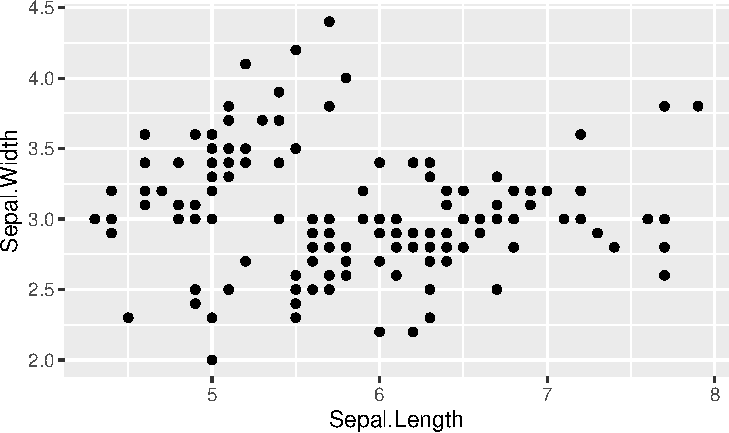
\includegraphics{final_project_template_files/figure-latex/unnamed-chunk-1-1} 

}

\caption{Example plot title}\label{fig:unnamed-chunk-1}
\end{figure}

\section{Citations in RMarkdown}\label{citations-in-rmarkdown}

\begin{itemize}
\item
  There is a .bib file in the GitHub ``Final Project'' folder that has
  the paper. You should input your references there. If you use a
  reference software, such as Zotero or Mendeley, there are options to
  export a bib file from it for your project or specific files as well.
\item
  To cite an article, write \texttt{@article\_key} such as Mandel and
  Semyonov (\citeproc{ref-mandel_going_2016}{2016}) or for parenthesis
  (\citeproc{ref-mandel_going_2016}{Mandel and Semyonov 2016:1045})
\item
  To edit the citation style, change the citation language style (CSL)
  specified in the YAML header.
\item
  RMarkdown will automatically add a references section at the end of
  your document.
\item
  For more information on RMarkdown references, see guides
  \href{https://bookdown.org/yihui/bookdown/citations.html}{here} and
  \href{https://bookdown.org/yihui/rmarkdown-cookbook/bibliography.html}{here}
\end{itemize}

\section*{References}\label{bibliography}
\addcontentsline{toc}{section}{References}

\phantomsection\label{refs}
\begin{CSLReferences}{1}{1}
\bibitem[\citeproctext]{ref-mandel_going_2016}
Mandel, Hadas, and Moshe Semyonov. 2016. {``Going {Back} in {Time}?
{Gender} {Differences} in {Trends} and {Sources} of the {Racial} {Pay}
{Gap}, 1970 to 2010.''} \emph{American Sociological Review}
81(5):1039--68. doi:
\href{https://doi.org/10.1177/0003122416662958}{10.1177/0003122416662958}.

\end{CSLReferences}

\end{document}
